\documentclass[a4paper,10pt, twocolumn]{article}
\usepackage[utf8]{inputenc}
\usepackage{amsmath}
\usepackage{amssymb}
\usepackage{amsthm}
\usepackage[usenames,dvipsnames]{color}
\usepackage{comment}
\usepackage{tikz}
\usepackage{verbatim}
\usetikzlibrary{arrows,shapes}
\usepackage{listings}
\usepackage{algorithm}
\usepackage{algpseudocode}
\usepackage{hyperref}
\usepackage{graphicx}
\usepackage{epstopdf}
\usepackage{tabularx}
\usepackage{enumitem}
\floatstyle{plaintop}
\usepackage{float}
\restylefloat{table}
\setlist{nolistsep}
\setlength{\parindent}{0cm}

%page boarders
\usepackage[top=3cm, bottom=3cm, left=2cm, right=2cm]{geometry}
\usepackage[style=numeric,backend=bibtex]{biblatex}
\addbibresource{../sources}
%\usepackage[style=mla,babel=hyphen,backend=biber]{biblatex}

\tikzstyle{vertex}=[circle,fill=black!25,minimum size=20pt,inner sep=0pt]
\tikzstyle{edge} = [draw,thick,->,>=latex,shorten >=1pt]
\tikzstyle{weight} = [font=\small]
\tikzstyle{selected edge} = [draw,line width=2pt,->,red!75,>=latex]
\tikzstyle{residual edge} = [draw,thick,->,blue!75,>=latex]
\tikzstyle{vertexE}=[circle,fill=black!25,minimum size=20pt,inner sep=0pt]

% Declare layers (for more convenience when drawing graphs)
\pgfdeclarelayer{background}
\pgfsetlayers{background,main}

\newtheorem{lemma}{Lemma}
\newtheorem{corollary}[lemma]{Corollary}
\newtheorem{theorem}[lemma]{Theorem}

\title{Parallel Network Flow Algorithms \\ 
\large A follow up seminar to the Parallel Algorithms lecture\footnote{Jesper Larsson Träff, lecture "Parallel Algorithms", 2012 winter term at TU Wien.}}
\author{Martin Kalany, 0825673}

\begin{document}
\maketitle

\section{Abstract}
\label{sec:abstract}
\textit{We discuss possibilities of parallelizing algorithms for the problem of finding a maximum flow in a given flow network. Although sequential algorithms have been known for a long time, efficient, poly-logarithmic parallel algorithms could not be found despite large efforts. Only in the 1990s theoretical analysis of the problem was able to ascertain the inherently sequential nature of the problem, i.e., that no parallel algorithm that solves the problem in poly-logarithmic time with polynomially bounded resource consumption exists, assuming that $NC \neq P$. After a detailed introduction to the problem and reviewing the algorithm of Ford and Fulkerson, we will prove the inherently sequential nature of the problem. Two fundamental parallel algorithms that nicely convey approaches of parallelization are presented and their asymptotic bounds are studied based on the PRAM model. We compare those two algorithms with later and improved algorithms, both sequential and parallel variants.}


\section{Introduction}
\label{sec:intro}
The \emph{maximum flow problem} (\lstinline|MAX-FLOW|), is an important problem in algorithms and graph theory with numerous applications\cite{ahuja93}. A detailed description of the problem is given in Section \ref{sec:networkFlows} along with definitions for all graph theoretical concepts used in this paper. Section \ref{sec:fordfulkerson}, to illustrate the problems and definitions, gives a quick explanation of the algorithm of Ford and Fulkerson, an intuitive sequential algorithm solving the problem. The PRAM model, which we will use as our model of computation in this paper, will briefly be described in Section \ref{sec:model}. In Section \ref{sec:cc} the inherently sequential nature of the problem will be shown. The informal term ``inherently sequential'' describes computational problems for which it is unlikely that efficient parallel algorithms with run time in $O(\log^{k}n)$ (for input size $n$ and some constant $k$) exist, although sequential algorithms $\in P$, i.e., with an asymptotic run time in $O(n^{k})$, are known.

Section \ref{sec:dinitz} discusses Dinitz' scheme, a fundamental result in graph theory that allows to  decompose the problem of finding a maximum flow in an arbitrary directed acyclic graph with $n$ vertices into $O(n)$ problems of finding a maximal flow in a layered network, which is a significantly simpler problem. Several improvements of previous algorithms are based on Dinitz' scheme, as is an early parallel algorithm of Shiloach and Vishkin, which will be presented in detail in  Section \ref{sec:shiloach}. This algorithm solves \lstinline|MAX-FLOW| in a layered network using the pre-flow push principle. Section \ref{sec:sv_parImpl} gives the necessary technical details for a parallel implementation of the algorithm, while Sections \ref{sec:sv_seq}, \ref{sec:sv_nr_procs} and \ref{sec:sv_analysis} deal with the theoretical analysis of the sequential variant\footnote{Simulating the parallel algorithm with one processor trivially yields a sequential algorithm.}, the number of required processors and the asymptotic complexity, respectively.

Another approach to solve the problem in parallel was developed by Goldberg and Tarjan. Their approach works on directed acyclic graphs without the detour via layered networks. It keeps track of the movement of each unit of flow by tracking it's path through the network. We will explain their solution in Section \ref{sec:goldberg} and provide theoretical analysis in Section \ref{sec:gt_analysis}. We finish our discussion with a comparison of the algorithms presented in this paper and further important results as well as some concluding remarks in Section \ref{sec:further}. 

\section{Network flows}
\label{sec:networkFlows}
A \textbf{flow network} \cite{ahuja93} is given by $N = (G,s,t,c)$, where
\begin{itemize}
	\item $G =(V,E)$ is a directed graph
    \item $s, t \in V$, $s \neq t$ are the source and terminal node
   	\item $c:E\rightarrow \mathbb{R}_0^{+}$ assigns a capacity $\forall e \in E$
   	\item $n=\lvert V\rvert$, $m=\lvert E\rvert$
\end{itemize}

Furthermore, the following assumptions are made:
\begin{itemize}
	\item $G$ is connected
	\item $G$ is simple, i.e., does not contain loops or parallel arcs
	\item There is no path $P(s,t)$ from source node $s$ to sink node $t$ with infinite capacity
\end{itemize}

\medskip
$f:E \rightarrow \mathbb{R}_0^{+}$ is a \textbf{flow} if it satisfies:
\begin{itemize}
	\item \emph{Capacity constraints:} $f(e) \leq c(e)$ $\forall e \in E$
	\item \emph{Flow conservation:} 
	$ \sum\limits_{u \in V} f(u,v) =  0 \Leftrightarrow \mathrm{IN}$\footnote{$\mathrm{IN}(f,v)$ and $\mathrm{OUT}(f,v)$ designate the amount of flow entering and exiting a node $v$}$(f,v) = \mathrm{OUT}(f,v)$ $\forall v \in V \setminus \{s,t\}$
	\item \emph{Skew symmetry:} $f(v,w) = -f(w,v)$
	\item \emph{Value of a flow:} $\lvert f\rvert := f(V,t)$ 
\end{itemize}

A flow $f$
\begin{itemize}
	\item is a \emph{maximum flow} if $\lvert f\rvert \geq \lvert f'\rvert$, for any other flow $f'$
	\item \emph{saturates} an arc e if $f(e) = c(e)$
	\item is a \emph{maximal (or blocking) flow} if every directed path P(s,t) contains at least one saturated arc
\end{itemize}
\medskip
The \emph{residual capacity} of $e \in V \times V$ w.r.t.\ a flow $f$ is defined as $c_r(e) = c(e) - f(e)$. $G_r = (V, E_r)$ is the \emph{residual network}, where $E_r = \left\{e \in V \times V \lvert c_r(e) > 0\right\}$. The set of \emph{admissible arcs} of a vertex $v$ is the set of all arcs $e$ emanating from $v$ s.t. $c_r(e) > 0$.  A path $P$ from $s$ to $t$ in $G_r$ is called an \emph{augmenting path} if it consists of admissible arcs only. An augmenting path $P(s,t)$ can be used to increase the flow $f$. Let $f_P(e)$ be the flow assigned to arc $e$ in augmenting path $P$. The flow $f$ can now be increased by $\forall e \in P: f(e) = f(e) + f_P(e)$.

\subsection{Algorithm of Ford-Fulkerson}
\label{sec:fordfulkerson}
The algorithm of Ford and Fulkerson as shown in Algorithm \ref{algo:fordFulkerson} is a sequential algorithm that solves \lstinline|MAX-FLOW|: starting from a null flow (or any other valid flow), increase the flow along an augmenting path as long as such a path exists. This is done by finding a path from $s$ to $t$ in the residual network along which the flow can be increased. 

\begin{algorithm}
\caption{Ford-Fulkerson}
\label{algo:fordFulkerson}
\begin{algorithmic}[1]
	\Function{Ford-Fulkerson}{$N=(G=(V,E),s,t,c)$}
	\State $f(u,v) = 0$ $\forall e=(u,v) \in E$ \Comment{Start with a valid flow}
	\State  $G_r = G$ 
	\State $c_r(P) = min \{c_r(u,v): (u,v) \in P(s,t) \}$
	\While{$\exists P(s,t) \in G_r: \forall (u,v) \in P(s,t): c_r(u, v) > 0$}
		\State $f(u,v) = f(u,v) + c_r(P)$ \Comment{Increase the flow by as much flow as can be pushed along $P(s,t)$}
		\State $c_r(u,v) = c_r(u,v) - c_r(P)$
		\State $f(v,u) = f(v,u) + c_r(P)$ 
	\EndWhile
	\EndFunction
\end{algorithmic}
\end{algorithm}

As an illustration of the algorithm, Figure \ref{fig:fordfulkerson1} depicts the flow network for which \lstinline|MAX-FLOW| is to be solved and the first augmenting path\footnote{The residual network is equal to the given network in the first step.}. Note that this path may be chosen arbitrarily. Figure \ref{fig:fordfulkerson2} shows the residual network resulting from the situation in Figure \ref{fig:fordfulkerson1} and a possible next augmenting path. 

Note that the algorithm of Ford and Fulkerson is restricted to integer capacities:  $c:E\rightarrow \mathbb{N}_0^{+}$ $\forall e \in E$. For a more detailed explanation and theoretical analysis, refer to \cite{ahuja93}.

\begin{figure}
\begin{center}
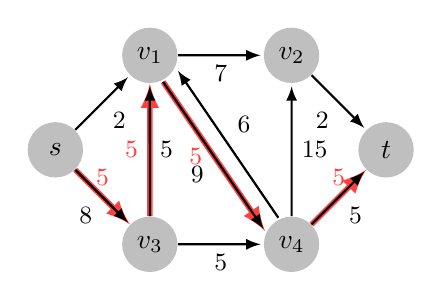
\begin{tikzpicture}[scale=1.2, auto,swap]
    % draw the vertices
	\foreach \pos/\name in {{(0,2)/s}, {(1,3)/v_1}, {(2.5,3)/v_2},
   	                        {(1,1)/v_3}, {(2.5,1)/v_4}, {(3.5,2)/t}}
    \node[vertex] (\name) at \pos {$\name$};
   	% Connect vertices with edges and draw weights
   	\foreach \source/ \dest /\weight in {s/v_1/2, s/v_3/8,v_3/v_1/5,
                                         v_1/v_2/7, v_4/v_2/15, v_3/v_4/5,
                                         v_2/t/2, v_4/t/5}
       	\path[edge] (\source) -- node[weight] {$\weight$} (\dest);
        	
       	%v_1/v_4/9
       	\path[edge] ([xshift= -4pt, yshift= 8pt] v_4.center) -- node[weight] {6}  ([xshift= 8pt, yshift= -4pt] v_1.center);
       	\path[edge] ([xshift = 4pt, yshift= -8pt] v_1.center) -- node[weight] {9}  ([xshift= -8pt, yshift= 4pt] v_4.center);
  
	% For convenience we use a background layer to highlight edges
   	% This way we don't have to worry about the highlighting covering
	% weight labels. 
	\begin{pgfonlayer}{background}
   	    \foreach \source /\dest  /\weight in {s/v_3/5,v_4/t/5}
	        \path[selected edge] (\source) -- node[weight,above] {$\weight$}(\dest);		
            \path[selected edge] ([xshift = 4pt, yshift= -8pt] v_1.center) -- node[weight,left] {5}  ([xshift= -8pt, yshift= 4pt] v_4.center);
            \path[selected edge] (v_3) -- node[weight,left] {$5$}(v_1);
   	\end{pgfonlayer}
\end{tikzpicture}
\end{center}
\caption{Algorithm of Ford-Fulkerson: Initial network (thin, black) and first augmenting path (thick, red)}
\label{fig:fordfulkerson1}
\end{figure}

\begin{figure}
\begin{center}
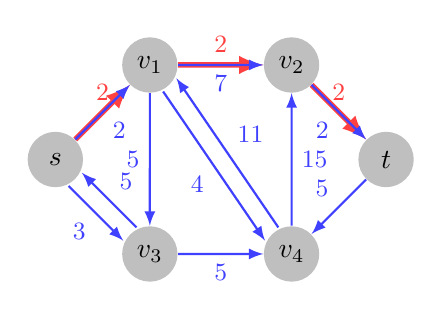
\begin{tikzpicture}[scale=1.2, auto,swap]
   	% draw the vertices
    \foreach \pos/\name in {{(0,2)/s}, {(1,3)/v_1}, {(2.5,3)/v_2},
    	                        {(1,1)/v_3}, {(2.5,1)/v_4}, {(3.5,2)/t}}
    \node[vertex] (\name) at \pos {$\name$};
   	% Connect vertices with edges and draw weights
   	\foreach \source/ \dest /\weight in {s/v_1/2, v_1/v_3/5, t/v_4/5,
                                         v_1/v_2/7, v_4/v_2/15, v_3/v_4/5,
                                         v_2/t/2}
       	\path[residual edge] (\source) -- node[weight] {$\weight$} (\dest);

        	%s/v_3/8,
       	\path[residual edge] ([xshift= -4pt, yshift= 8pt] v_3.center) -- node[weight] {5}  ([xshift= 8pt, yshift= -4pt] s.center);
       	\path[residual edge] ([xshift = 4pt, yshift= -8pt] s.center) -- node[weight] {3}  ([xshift= -8pt, yshift= 4pt] v_3.center);
        	%v_1/v_4/9
       	\path[residual edge] ([xshift= -4pt, yshift= 8pt] v_4.center) -- node[weight] {11}  ([xshift= 8pt, yshift= -4pt] v_1.center);
       	\path[residual edge] ([xshift = 4pt, yshift= -8pt] v_1.center) -- node[weight] {4}  ([xshift= -8pt, yshift= 4pt] v_4.center);       	
        	
       	\begin{pgfonlayer}{background}
   	    \foreach \source /\dest  /\weight in {s/v_1/2,v_1/v_2/2,v_2/t/2}
            \path[selected edge] (\source) -- node[weight,above] {$\weight$}(\dest);			            
   	\end{pgfonlayer}
\end{tikzpicture}
\end{center}
\caption{Algorithm of Ford-Fulkerson: Residual network (thin, blue) and augmenting path (thick, red)}
\label{fig:fordfulkerson2}
\end{figure}	

\section{Model of Computation}
\label{sec:model}
We use the \textbf{PRAM} Model\footnote{Parallel Random Access Machine, as defined in the lecture or in \cite{papa95}.} as the model of computation. The PRAM model is a high level abstraction of a shared memory machine, in which memory access by any processor to any memory location is assumed to require constant time. Specifically, a \textbf{MIMD} (Multiple Instructions Multiple Data) variant is used, where each processor $p$ executes a distinct set of instructions on distinct data. Instructions are executed in lock-step and any necessary padding of instructions is assumed to be done automatically. 

\section{Computational Complexity}
\label{sec:cc}
The algorithmic complexity of the \emph{Ford-Fulkerson} algorithm is given as $O((n+m)f_{\mathrm{max}})$\footnote{$f_{\mathrm{max}}$ is from here on used to denote the maximum flow.} \cite{ahuja93,papa95}. This was improved by the \emph{Edmonds-Karp} algorithm to $O(nm^2)$, by using shortest augmenting paths instead of arbitrarily chosen ones. Clearly, the \emph{maximum flow problem} can be solved in polynomial time with a sequential algorithm and thus \lstinline|MAX-FLOW| $\in P$.

Informally, algorithms may be \emph{efficiently parallelizable} or \emph{inherently sequential}. The complexity class \textbf{NC} \cite{papa95} ("Nick's Class") contains all problems solvable in $O(\log^{k_1}(n))$ time and $O(n^{k_2})$ total work. We give a useful alternate definition:  A language that is decided by PRAM in $O(\log^{k_1}(n))$ time steps with $O(n^{k_2})$ processors available at each step is in $NC$. Problems in $NC$ thus are solvable  in poly-logarithmic time requiring polynomial work (or resources, such as processors and memory). Problems in $P \setminus NC$ are dubbed "inherently sequential", i.e., not parallelizable efficiently. 

Clearly, $NC \subseteq P$, but whether $NC \subset P$ or $NC = P$ is still unknown. It follows that we do not know whether or not inherently sequential problems actually exist. The most likely problems to be hard to parallelize are problems that are P-complete w.r.t.\ NC reduction. Since any problem $A \in P$ can be reduced to a P-complete problem $B$, a parallel algorithm that solves $B$ within poly-logarithmic time bounds would immediately imply that for all problems $\in P$ a parallel algorithm $\in NC$ exists \cite{papa95}.

As an example, the Ford-Fulkerson algorithm can not be parallelized trivially. Although constructing the residual network can be done in constant time $O(1)$ (by assigning a processor to each arc $e \in E$) and augmenting paths can be found in $O(\log^{2}n)$ time and $O(n^{2})$ work by a basic breath first search, the number of stages can not be reduced to less than $O(\sqrt{n})$ \cite{ahuja93}. Thus the total complexity, which is dominated by the number of stages, places the algorithm in $P \setminus NC$.
	
As shown in \cite{papa95}, \lstinline|MAX-FLOW| is P-complete and no parallel algorithm $\in NC$ is currently known for solving this problem. It is assumed that the problem is inherently sequential\footnote{provided that $P \neq NC$.}.

\section{Dinitz' scheme}
\label{sec:dinitz}
$N = (V,E,s,t,c)$ is a \textbf{layered network} \cite{yossi81} if each vertex $v \in V$ has a layer number $l(v)$ s.t.
\begin{itemize}
	\item $l(s) = 0$ and $0 \leq l(v) \leq l(t)$ $\forall v \in V$
	\item $e = (u,v) \in E  \Rightarrow l(v) - l(u) = 1$
\end{itemize}
Figure \ref{fig:dinitz} shows a layered network and it's underlying directed acyclic network.

\begin{figure}
\begin{center}
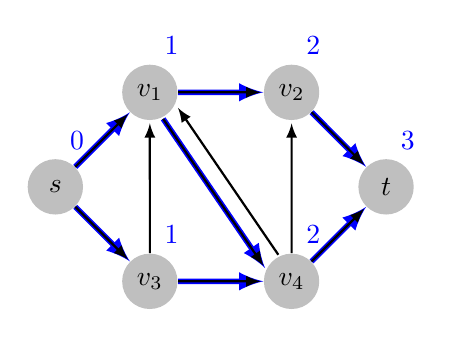
\begin{tikzpicture}[scale=1.2, auto,swap]
   	% draw the vertices
	\foreach \pos/\name/\layer in {{(0,2)/s/0}, {(1,3)/v_1/1}, {(2.5,3)/v_2/2},
    	                        {(1,1)/v_3/1}, {(2.5,1)/v_4/2}, {(3.5,2)/t/3}}
    \node[vertex,label={[color=blue]80:$\layer$}] (\name) at \pos {$\name$};
        
    %\node[vertex,label={[color=blue]80:$+12$}] (v_1) at (1.5,3) {$v_1$};
    % Connect vertices with edges and draw weights
    \foreach \source/ \dest in {s/v_1, s/v_3,v_3/v_1,
                                        v_1/v_2, v_4/v_2, v_3/v_4,
                                        v_2/t, v_4/t}
     \path[edge] (\source) -- (\dest);
        	
     %v_1/v_4/9
     \path[edge] ([xshift= -4pt, yshift= 8pt] v_4.center) -- ([xshift= 8pt, yshift= -4pt] v_1.center);
     \path[edge] ([xshift = 4pt, yshift= -8pt] v_1.center) -- ([xshift= -8pt, yshift= 4pt] v_4.center);
  
	% For convenience we use a background layer to highlight edges
    % This way we don't have to worry about the highlighting covering
	% weight labels. 
	\begin{pgfonlayer}{background}
    	\foreach \source /\dest in {s/v_3,v_2/t,s/v_1,v_1/v_2,v_3/v_4,v_4/t}
	      	\path[selected edge, color=blue] (\source) -- (\dest);		
	    \path[selected edge, color=blue] ([xshift = 4pt, yshift= -8pt] v_1.center) -- ([xshift= -8pt, yshift= 4pt] v_4.center);
	\end{pgfonlayer}
\end{tikzpicture}
\end{center}
\caption{A layered network (in blue) with layer numbers and it's underlying network}
\label{fig:dinitz}
\end{figure}

\begin{theorem}
\textbf{Dinitz' scheme} \cite{dinitz70} \\
A maximum flow problem in a general network can be transformed into $O(n)$ maximal flow problems in layered networks.
\end{theorem}

A layered network can easily be constructed from a directed acyclic network by performing breath-first search, which can be done in parallel in $O(\log^{2}n)$ time\cite{yossi81}. It follows that an algorithm that finds a maximal/blocking flow in a layered network can solve \lstinline|MAX-FLOW| in $O(n)$ iterations. The basic scheme is given in Algorithm \ref{algo:dinitz}.

\begin{algorithm}
\caption{Dinitz' scheme}
\label{algo:dinitz}
\begin{algorithmic}[1]
	\Function{MAX-FLOW}{$N=(V,E,s,t,c)$}
	\State start with some valid flow 
	\While{$l(t) \neq \infty$} %\Comment{\textcolor{OliveGreen}{$O(n)$}}	
		\State Construct residual network $G_r$ %\Comment{\textcolor{OliveGreen}{$O(n)$, $p=O(n)$}}
		\State Construct layered network $G_l$ from $G_r$ %\Comment{\textcolor{OliveGreen}}{$O(m/p + n)$}
		\State $f_l$ = MAX-FLOW($G_l$)  %\Comment{tbd}
		\State $f$ = $f$ + $f_l$ %\Comment{\textcolor{OliveGreen}{$O(n)$}}
	\EndWhile
	\EndFunction
\end{algorithmic}
\end{algorithm}

\section{Algorithm of Shiloach and Vishkin}
\label{sec:shiloach}
The Shiloach-Vishkin algorithm is based on Dinitz' scheme as shown in Section \ref{sec:dinitz}. This section focuses on the implementation of an algorithm to solve \lstinline|MAX-FLOW| for a given layered network.

The following notation will be used:
\begin{description}
	\item [EXCESS(v)] The amount of excessive pre-flow at node $v$. \lstinline|EXCESS(v)| = $\mathrm{IN}(f,v) - \mathrm{OUT}(f,v) \geq 0$.
	\item[UNBALANCED] The set of vertices that hold some excess flow. \lstinline|UNBALANCED| = $\{v \in V \lvert \mathrm{EXCESS}(v) > 0 \}$. The sequential implementation (Section \ref{sec:sv_seq}) uses a queue to maintain FIFO order on the set of unbalanced vertices.
	\item[blocked] A vertex v is blocked if for all it's outgoing arcs $e_i = (v, u_i)$, $e_i$ is either saturated or $u_i$ is blocked\footnote{The sink vertex $t$ is never blocked.}. 
\end{description}
	
The algorithm operates in \emph{pulses}: In the first pulse, all outgoing arcs of $s$ or saturated: $\forall e_i = (s, v_i):$ $f(e_i) = c(e_i)$. The set of unbalanced vertices at the end of pulse 1 is thus the set of all neighbors of $s$: \lstinline|UNBALANCED| = $\{v_i\lvert \exists (s, v_i) \in E \}$. In each subsequent pulse, the unbalanced vertices try to push forward\footnote{i.e., to the next layer of the network.} as much of their excessive flow as possible. Any remaining excessive flow will be returned backwards. All balanced vertices remain idle during the pulses. The algorithm terminates as soon as no unbalanced vertices are available, implying that all flow reached the source $s$ or sink $t$.

Algorithm \ref{algo:sv} shows an abstract routine for solving \lstinline|MAX-FLOW| in a given layered network. In each pulse $p>1$, the \lstinline|while| loop in lines 4-12 is executed in parallel for each node $v \in \mathrm{UNBALANCED}$. Parallel implementations of functions \lstinline|PUSH| and \lstinline|RETURN| are depicted in Algorithm \ref{algo:sv_push} and Algorithm \ref{algo:sv_return}, respectively and will be explained in detail in the remainder of this section. The algorithm maintains the number of the current pulse in \texttt{i}.

\begin{algorithm}
\caption{Shiloach-Vishkin}
\label{algo:sv}
\begin{algorithmic}[1]
	\Function{MAX-FLOW}{$G_l$}
		\State EXCESS(s) = $\Sigma_{v \in L_1}$ c(s$\rightarrow$v)
		\State PUSH(s, EXCESS(s))
		i = 1;
		\While{$\exists$ v $\in UNBALANCED$}
			\State i++
			\ForAll {$v \in UNBALANCED$}			
				\If{$v$ is not blocked}
					\State PUSH(v, EXCESS(v))
				\EndIf
			\EndFor
			\State RETURN(v, EXCESS(v))
		\EndWhile
	\EndFunction
\end{algorithmic}
\end{algorithm}

\subsection{Partial Sums trees}
\label{sec:sv_pstrees}
A \emph{partial sums tree} (PS-tree) is a complete binary tree with the leftmost $k$ leaves associated with $k$ numbers $a_1,...,a_k$. A PS-tree is of height $height := \lceil \log_2(k) \rceil$ and has $width := 2^{\lceil \log_2(k) \rceil}$ leaves. The remaining $w - k$ rightmost leaves are associated with 0. Each internal node of a PS-tree stores the sum of it's child nodes. Thus, the root node stores the sum of all the leaves of the tree. Figure \ref{fig:pstree} provides an example.

\begin{figure}[H]
\begin{center}
  \begin{tikzpicture}[scale=0.8,label distance=-3mm,>= latex, node distance = 2cm,level/.style={sibling distance=40mm/#1}]
    \tikzstyle{every node}=[draw=none,fill=none, minimum size=5mm,font=\footnotesize];

   \node (pr) {$23$}
   	child {node (p13) {$17$}
	  	child {node (p9) {$8$} 
    	 	child {node (p1) {$5$}}
      		child {node (p2) {$3$}}
    		}
  		child {node (p10) {$9$} 
    	  	child {node (p3) {$2$}}
      		child {node (p4) {$7$}}
   		 }
   	}
   	child {node (p14) {$6$} 
   		child {node (p11) {$6$} 
      		child {node (p5) {$6$}}
		    child {node (p6) {$0$}}
    		}
   		child {node (p12) {$0$} 
      		child {node (p7) {$0$}}
      		child {node (p8) {$0$}}
      	}
    };
\end{tikzpicture}
\end{center}
\caption{A partial sums tree with $k=5$}
\label{fig:pstree}
\end{figure}

A \emph{flow quantum} is a 3-tuple $(p, e, f)$, where $p$ is the number of the pulse during which some flow of value $f$ reached a vertex $v$ via arc $e$.

For the parallel implementation of \lstinline|PUSH| and \lstinline|RETURN|, several PS-trees will be used. Four PS-trees are attached to every vertex $v \in V$:
\begin{description}
	\item [T-OUT($v$)] Each active leaf $a_i$ is associated with an outgoing arc $e_i = (v, w_i)$. The value of leaf $i$ is $a_i = c(e_i) - f(e_i)$, i.e., $a_i$ stores the residual capacity of $e_i$. T-OUT($v$) has $d_{\mathrm{out}}(v)$\footnote{As usual, $d_{\mathrm{in}}(v)$ and $d_{\mathrm{out}}(v)$ designate the in- and out-degree of a vertex.} active leaves.
	\item [T-IN($v$)] Records flow quanta reaching $v$. T-IN($v$) has $2nd_{\mathrm{in}}(v)$ active leaves to be able to record the pulse\footnote{the number of pulses is bounded by $O(2n)$ \cite{yossi81}.} and arc for each flow quantum that reaches $v$. 
	\item [T-ACCESS($v$)] Each of the $d_{\mathrm{in}}(v)$ active leaves is associated with one edge entering $v$. Used to coordinate access to $v$.
	\item [T-SUM($v$)] Sums up the flow returned to $v$ in a given pulse. $d_{\mathrm{out}}(v)$ active leaves. 
\end{description}
One PS-tree is attached to every arc $e \in E$:
\begin{description}
	\item [T-EDGE($e$)] $2n$ active leaves, each of which is associated with one pulse to record the amount of flow returned on $e$ in a given pulse.
\end{description}

Let T be a PS-tree. Every node of T is represented by $T[height, i]$. We use $root$ as index for the root node of T. Thus, $height(T[root]) := \lceil \log_2(k) \rceil$ and $height(a_i) := 1$ , $\forall$ leaves $a_i$.  We define the following operations on T:
\begin{description}
	\item [CLEAR($i$)] The value of all nodes on the path $P(T[1,i],root)$ is set to 0. 
	\item [UPDATE($i$, $a_i$)] The value of the i-th leaf is set to $a_i$ and the values of all nodes on the path $P(T[1,i],root)$ are updated.
	\item [SUM($i$, $S_i$)] Calculate the sum of values stored in leave nodes $a_1...a_i$. $S_i = a_1,...,a_i$.
	\item [FIND($\alpha$, $k$, $\rho$)] Given $\alpha$, find $k$ and $\rho$ s.t. $a_1+...+a_{k-1} < \alpha \leq a_1+...+a_k$ and $\rho = \alpha - (a_1+...+a_{k-1})$. Given an amount of flow $\alpha$, this operation will be used to find the number $k$ of edges required to push flow from a node $v$. Along the first $k-1$ edges an amount of flow equal to the residual capacity of each each will be pushed. The remaining amount of flow $\rho$ will be pushed along edge $k$. 
\end{description}

\begin{theorem}
CLEAR, UPDATE, SUM and FIND each require $O(\log n)$ time steps on a CRCW PRAM with common write ability\cite{yossi81}.
\end{theorem}
\begin{proof}
Of the 5 PS-trees defined above (T-OUT(v), T-IN(v), T-ACCESS(v), T-SUM(v) and T-EDGE(e)), T-IN(v) has the most active leaves: $2nd_{\mathrm{in}}(v) \leq 2n^2$. This implies height of $2 \lceil \log n \rceil$ for the complete binary tree, which is bounded by $O(\log n)$. All operations work on paths from some leaf $a_i$ to the root of the tree. Implementing them as follows ensures a time complexity of $O(\log n)$ for all operations on a CRCW PRAM. In particular, a \emph{common write} variant is required, where all processors attempting to write to the same memory location have to write the same value.
\begin{description}
	\item [FIND] does a binary search from the root node of the tree $T[root]$ to leaf $i$, s.t. $a_{i-1} < \alpha \leq a_i$. 
	\item [SUM] On the path $P(T[root], i)$, sum up the values of left child nodes when traversing to the right child node and add the value $a_i$.
	\item [CLEAR] Sets the values of nodes on the path $P(i, T[root])$ to 0. Note that this would potentially invalidate the PS-tree. However, this operation will be executed for all leaves of the tree simultaneously, thus clearing the whole tree. Resulting PRAM requirements will be discussed below.
	\item [UPDATE] Updates the value of leaf $i$ followed by the values of all nodes on the path $P(i, T[root])$. To do so, for all nodes along $P(i, T[root])$ the values of both children need to be accessed.
\end{description}
\end{proof}

The original paper\cite{yossi81} claims that:
\begin{theorem}
The same performance can be achieved using a CREW PRAM.
\end{theorem}

Unfortunately, this far from trivial claim is not further elaborated on in the paper. It is easy to achieve for the CLEAR operation: starting at the leaves of the tree, at each level every second processor can stop. The processor doing the update on the sibling node will take care of the remaining nodes, since they share the same path to the root. 

A similar scheme may be devised for operations on T-OUT($v$): All $p$ processors will operate on $p$ consecutive leaf nodes of the tree (this is implied by the PUSH function). However, this is not true for UPDATE operations on T-IN($v$): during one pulse, the incoming flow may be pushed to $v$ along any subset of $d_{\mathrm{in}}(v)$, requiring UPDATE for some leaves within a range of 2n. We were not able to reproduce the claim for this situation. 

\subsection{Parallel Implementation}
\label{sec:sv_parImpl}
We use the following processor assignment:
\begin{itemize}
	\item Each vertex $v \in V$ has a processor $P(v)$ assigned
	\item Each arc $e \in E$ has a processor $P(e)$ assigned
	\item Each flow quantum $Q$ has a processor $P(Q)$ assigned. In other words, each leaf in each of the $2n * d_{\mathrm{in}}(v)$ T-IN(v) PS-trees has a processor $P(Q)$ assigned.
\end{itemize}

The total number of required processors is $O(nm)$, which is dominated by the assignment of one processor for each flow quantum. This apparently large number of required processors can be reduced to $n$, which we will prove in Section \ref{sec:sv_nr_procs}. We will however use the above assignment of processors to present the essentials of the algorithm in cleaner way.   

In addition to the four PS-trees attached to each vertex $v$, $v$ keeps two pointers:
\begin{description}
	\item [head($v$)] Points to the rightmost significant leaf in T-in($v$). The rightmost significant leaf (i.e., the rightmost leaf with a value $\neq 0$) is associated with the flow quantum that was the last to reach $v$. head($v$) will be used to keep track of the order of flow quanta reaching a node $v$, in order to be able to return excess flow. 
	\item [$k'$] The outgoing arcs of $v$ are assumed to be ordered arbitrarily. $k'$ points to the first outgoing arc\footnote{the arc with the smallest index w.r.t. the given ordering.} that is not yet saturated. In other words, $k'$ points to the next arc that can be utilized to push excess flow from $v$.  
\end{description}

In Algorithms \ref{algo:sv_init}, \ref{algo:sv_push} and \ref{algo:sv_return}, the notation \textcolor{blue}{P():} is used to indicate that the following instructions are carried out only by the specified processors. Algorithm \ref{algo:sv_init} shows the initialization routine executed at the beginning of each pulse. Each processor assigned to an arc $e_j = (v, w)$ updates the PS-tree T-OUT attached to $v$ s.t.\ it's leave $a_j$ is assigned the residual capacity of $e_j$. $f(e_j$) is set to 0. In the next step, each processor assigned to a vertex $v$ initializes its pointers head($v$) and $k'(v)$.

\begin{algorithm}
\caption{Shiloach-Vishkin: INITIALIZE}
\label{algo:sv_init}
At beginning of each pulse:	
\begin{algorithmic}[1]
	\Function{INITIALIZE}{v}
		\State \textcolor{blue}{P($e_j = v \rightarrow w$):}
		\State UPDATE($j$, $c_r(e_j)$) T-OUT(v)
		\State f($e_j$) = 0
		\State \textcolor{blue}{P(v):}
		\State head(v) = 0	
		\State k'(v) = 1	
 	\EndFunction
\end{algorithmic}
\end{algorithm}

The \lstinline|PUSH| function is given in Algorithm \ref{algo:sv_push}. In lines 3-4, the amount of flow to be pushed in this pulse from node $v$ is calculated and the amount of excess flow remaining at node $v$ is updated. In line 5, the algorithm computes the number $k-1$ of outgoing arcs that will be saturated in this pulse, starting with the arc pointed to by $k'$, as well as the amount of flow $\rho$ that will be pushed on the k-th outgoing arc, without saturating that arc.

In the next step, all processors assigned to an arc $e_j$ s.t. $k'\leq j \leq k'+k$ will update their arc: In line 10, the flow of the k-th arc is updated by an amount $\rho$; in line 12, $k-1$ arcs are updated with as much flow as can be pushed through them. Lines 8-9 are used to count and order the processes that require access to node $w$, in order to store the flow quanta pushed to $w$ (line 16). In line 18, the \lstinline|head| pointer of node $w$ is advanced to the last recorded flow quantum. Lines 15 and 20 calculate the amount of excess flow at node $w$ (which is the amount of flow that was pushed to $w$ in this pulse). Finally, in lines 23-26 all vertices $v$ that have some remaining excess flow are blocked. Since no more flow can be pushed along their outgoing arcs, the remaining excess flow will have to be returned.

\begin{algorithm}
\caption{Shiloach-Vishkin: PUSH}
\label{algo:sv_push}
\begin{algorithmic}[1]
	\Function{PUSH}{v,EXCESS(v)}
		\State \textcolor{blue}{P(v):}
		\State $\alpha$ = min\{EXCESS(v), T-OUT(v)[root]\} 
		\State EXCESS(v) = EXCESS(v) - $\alpha$
		\State FIND($\alpha$, k, $\rho$) in T-OUT(v)
		\State \textcolor{blue}{P($e_j = v \rightarrow w$):}
		\If{k' $\leq$ j $\leq$ k' + k}
 		\State UPDATE(j,1) in T-ACCESS(w)
		\State SUM(j,$S_j$) in T-ACCESS(w)
		\If{$j == k$}
			$q_j$ = $\rho$
		\Else
			\State $q_j$ = T-OUT(v)[1,j]
		\EndIf
		\State $f(e_j)$ = $f(e_j)$ + $q_j$
		\State TOTAL(w) = T-IN(w)[root]
		\State UPDATE(head(w) + $S_j$, $q_j$) in T-IN(w)
		\State UPDATE(j, T-OUT(v)[1,j] - $q_j$) in T-OUT(v)
		\State head(w) = head(w) + T-ACCESS(w)[root] 
		\State CLEAR(j) in T-ACCESS(w)
		\State EXCESS(w) = T-IN(w)[root] - TOTAL(w)
		\EndIf
		\State \textcolor{blue}{P(v):} k' = k
		\State \textcolor{blue}{P($e_j = v \rightarrow w$):}
		\If{EXCESS(v) $>$ 0}
			\State block v
		\EndIf
 	\EndFunction
\end{algorithmic}
\end{algorithm}

The \lstinline|RETURN| function given in Algorithm \ref{algo:sv_return} returns any excessive flow remaining at a node $v$. The excessive flow at node $v$ is the amount of flow that was pushed to $v$ but could not be pushed further along any of the outgoing arcs $e_j$ of $v$. This is the case when for all outgoing arcs $e_j = (v ,w_j)$ of $v$ at least one of two conditions hold: either the arc $e_j$ is saturated or the node $w_j$ is blocked. 

The algorithm works as follows: In line 3, we find the number $k$ of arcs into node $v$ that carry the flow that was pushed to $v$ and than further along outgoing arcs of $v$. Note that this amount of flow constitutes a valid flow through node $v$, satisfying all requirements of a flow as given in Section \ref{sec:networkFlows}. Line 4 sets the amount of excessive flow at node $v$ to 0 (any excessive flow will be taken care of in the following steps).

In lines 5-9 the excess flow that will be returned on arcs $e_j$ s.t. $k \leq j \leq head(v)$, which brought the excess flow to $v$, is calculated. All arcs $e_j$ s.t. $k<j \leq head(v)$ will return as much flow as was pushed along them in any of the previous steps, resulting in 0 units of flow being pushed along them in the final flow of the given layered network. Arc $e_k$ will return an amount of flow of $d_k = q_k - \rho$, where $0 <= d_k <= c(e_k)$. Note that $\rho$ is the amount of flow that was pushed into node $v$ along arc $e_k$ and then pushed further along an outgoing arc of $v$. Thus, on $e_k$ only flow exceeding $\rho$, if any, has to be returned. In lines 8-9, the flow assigned to arcs $a_j$, which is the flow pushed into $v$ along arcs $e_j$, is updated accordingly.

Line 10 records the amount of flow that is returned on arc $e_j$ in this pulse. In line 11 the amount of flow assigned to arc $e_j$ is then reduced by the amount that was returned in this pulse. Note that \lstinline|T-EDGE|($e_j$)[root] contains the amount of flow returned on the current pulse only (not the sum of flow returned in all pulses so far since it is cleared at the end of each pulse in line 14).

In line 12, the amount of flow returned to node $u$ in the current pulse is calculated. This is done by storing the amount of flow that is returned to node $u$ via arc $e_j$ in the corresponding leave of \lstinline|T-SUM| by applying the \lstinline|UPDATE| function. The root node of \lstinline|T-SUM| then contains the sum of flow returned to node $u$ via all of its outgoing arcs. The returned flow will be excessive flow at node $u$ (since \lstinline|PUSH| pushed as much flow as possible along $u$'s outgoing in previous pulses) and will have to be taken care of in the next pulse. Thus, the amount of excessive flow at node $u$ is increased by the amount of flow returned to $u$.

Lines 14 and 15 simply clear \lstinline|T-EDGE| and \lstinline|T-SUM|, since their leaves are associated with pre-flow moved in the current pulse, as their definition in Section \ref{sec:sv_parImpl} states.

Finally, in line 17 the pointer $head$ is set to the latest flow quantum that was pushed into $v$ but not returned.

\begin{algorithm}
\caption{Shiloach-Vishkin: RETURN}
\label{algo:sv_return}
\begin{algorithmic}[1]
	\Function{RETURN}{v, EXCESS(v)}
		\State \textcolor{blue}{P(v):}
		\State FIND (T-IN(v)[root] - EXCESS(v), k, $\rho$) in T-IN(v)
		\State EXCESS(v) = 0
		\State \textcolor{blue}{$P(Q_j = (e_j = u \rightarrow v, q_j))$:}
		\State $d_j = q_j$ for $k < j \leq head(v)$
		\State $d_j = q_j - \rho$ if $j == k$
		\State UPDATE(j, 0) in T-IN(v) for $k < j \leq head(v)$
		\State UPDATE(j, $\rho$) in T-IN(v) if $j == k$
		\State UPDATE($p_j$,$d_j$) in T-EDGE($e_j$)
		\State $f(e_j)$ = $f(e_j)$ - T-EDGE($e_j$)[root]
		\State UPDATE($e_j$, T-EDGE($e_j$)[root]) in T-SUM(u)
		\State EXCESS(u) = EXCESS(u) + T-SUM(u)[root]
		\State CLEAR($r_j$) in T-EDGE($e_j$)
		\State CLEAR($e_j$) in T-SUM(u)
		\State \textcolor{blue}{P(v):}
		\State head(v) = k
	\EndFunction
\end{algorithmic}
\end{algorithm}

\subsection{Complexity of sequential algorithm}
\label{sec:sv_seq}
The parallel algorithm presented above can easily be turned into a sequential algorithm by executing it with only one processor: this one processor handles all vertices that are unbalanced at the beginning of a pulse, one at a time in an arbitrary order. However, the order of unbalanced vertices of different pulses needs to be enforced. A simple queue thus suffices to implement the set of unbalanced vertices \lstinline|UNBALANCED| used in Algorithm \ref{algo:sv}.

\begin{lemma}
The complexity of the sequential algorithm is $O(n^{3})$\cite{yossi81}.
\end{lemma}
\begin{proof}
All the elementary operations of the algorithm will be associated to either arcs or (vertex, pulse) pairs s.t. each arc or pair is assigned only a constant number of elementary operations. As shown in great detail by Shiloach and Vishkin in \cite{yossi81}, the number of pulses is bounded by $2n$, which implies an $O(n^{2})$  bound\footnote{Note that since $m < n^2$, the $m$ term is dominated by the $n$ term.} for the number of (vertex, pulse) pairs for one layered network, yielding a complexity of $O(n^{3})$ for the whole algorithm.

\begin{itemize}
	\item If an arc $e$ becomes saturated during a \emph{PUSH(v, EXCESS(v))}, the resulting operations (which are a constant number) are charged to $e$. In each pulse $p_i$ only one arc $e$ emanating from a vertex $v$ will be used to push along flow without $e$ becoming saturated and thus the elementary operations are charged to the corresponding pair $(v, p_i)$. This implies a bound of $O(n^2)$ elementary operations involved in all PUSH operations required to solve the \lstinline|MAX-FLOW| problem in a layered network.
	\item The elementary operations of \emph{RETURN(v, EXCESS(v)} will be charged either to related PUSH operations or again to a (vertex, pulse) pair. When some flow is returned from vertex $v$ at pulse $p_i$, the flow cancels out flow quanta that were pushed to $v$ at some pulse $p_j$ with $j \leq i$ and the corresponding push-operation is charged. The returned flow may furthermore cause a change in at most one flow quantum, in which case the elementary operations are assigned to the pair $(v, p_i)$. By the same argument as before, we get an $O(n^{2})$ bound on the number of elementary operations involved in all RETURN operations.
\end{itemize}

These charging rules yield an $O(n^{2})$ bound on the number of elementary operations involved in pushing and returning flow while solving \lstinline|MAX-FLOW| for a layered network, which implies an overall complexity of $O(n^{3})$ for the whole algorithm. 
\end{proof}

\subsection{Processor efficient parallel implementation}
\label{sec:sv_nr_procs}
\begin{theorem}
An allocation of processors to jobs s.t. $n$ processors are sufficient is possible without affecting the complexity of the algorithm. 
\end{theorem}
\begin{proof}
The \emph{Work-time framework} as presented in \cite{vishkin92} allows for a simple justification of the theorem. The number of rounds is $O(n^2 \log n)$: One pulse can be executed in $O(\log n)$ time steps (no loops, operations on binary trees of height $\lceil 2 \log 2n \rceil$ only). Since we need at most $2n$ pulses\footnote{see \cite{yossi81} for a detailed proof.} for solving \lstinline|MAX-FLOW| each of the $O(n)$ layered networks\footnote{according to Dinitz' scheme, as explained in Section \ref{sec:dinitz}.}, the total number of time steps is $T \in O(n^{2} \log n)$. By similar arguments as we used in Section \ref{sec:sv_seq}, we obtain an amount of total work $W \in O(n^{3} \log n)$\footnote{see \cite{yossi81} for a more detailed proof.}. Applying \emph{Brent's theorem}\cite{Brent74}, we get $\lceil W/p \rceil + T$ rounds, which is $O(n^{2} \log n)$ rounds for $p=n$, proving the lemma.
\end{proof}

\subsection{Analysis}
\label{sec:sv_analysis}
\begin{theorem}
The algorithm of Shiloach and Vishkin solves \lstinline|MAX-FLOW| in  $O(n^{2} \log n)$, using $O(n)$ processors on a CREW PRAM.
\end{theorem}

Using the results from the previous sections, we can now provide asymptotic bounds for all steps of Algorithm \ref{algo:sv}. According to Dinitz' scheme, the while-loop is bounded by $O(n)$ iterations. Constructing the residual network $G_r$ can trivially be done in $O(n)$ using $n$ processors, since $m \in O(n^{2})$. Breath-first search can be used to construct a layered network $G_l$ out of $G_r$. Efficient parallel implementations of BFS run in $O(m/p +n)$ time using n processors on a CREW PRAM\cite{Varman87}. Adding the found \lstinline|MAX-FLOW| of a layered network to the global \lstinline|MAX-FlOW| can again be done in $O(n)$ time. 

It remains to compute the complexity of finding a \lstinline|MAX-FlOW| in a layered network $G_l$, as shown in Algorithm \ref{algo:sv}. Each \lstinline|PUSH| or \lstinline|RETURN| operation requires $O(\log n)$ steps, since they do not contain any loops and statements operate on paths from a leaf to the root of a binary tree of height $O(\lceil \log_2(n) \rceil)$.

It follows that each round is executed in $O(n \log n)$ time, solving \lstinline|MAX-FLOW| for a layered network. Thus the algorithm overall has a time complexity of $O(n^{2} \log n)$. As shown in Section \ref{sec:sv_pstrees}, a CRCW PRAM is required for the operations on PS-trees. The claim of Shiloach and Vishkin\cite{yossi81}, that a CREW PRAM is sufficient to execute the algorithm within the given bounds could not be reproduced, as explained in Section \ref{sec:sv_pstrees}.

\section{Algorithm of Goldberg and Tarjan}
\label{sec:goldberg}
The Goldberg-Tarjan algorithm solves \lstinline|MAX-FLOW| on directed acyclic graphs. Contrary to the Shiloach-Vishkin algorithm presented in Section \ref{sec:shiloach}, it is not based on Dinitz' scheme (see Section \ref{sec:dinitz}). The algorithm constructs a blocking flow by moving flow through the network while maintaining a blocking pre-flow. Intuitively, the flow quanta do a depth-first search from $s$ to $t$ in a dynamic graph, where arcs become saturated and vertices become blocked.

\subsection{Atoms}
\label{sec:gt_atoms}
An \emph{atom} $a$ is defined as the maximal quantity of flow that so far moved along the same path $P(s,v)$. An atom $a$ can move forwards along an arc $e \in E$, or backwards along the same arc. Formally, the backward arcs are defined as $E^{-1} = \{(w,v)\vert (v,w) \in E \}$. Furthermore, an atom $a$ has the following properties:
\begin{description}
	\item [size($a$)] The amount of excess flow that $a$ carries.
	\item [position($a$)] The vertex $v \in V$ the atom $a$ is currently located at.
	\item [trace($a$)] The trace, i.e., the sequence of arcs the atom $a$ moved so far: $P_t(s, \mathrm{position}(a))$ in $E \cup  E^{-1}$. 
	\item [path($a$)] The simple Path $P_s(s, \mathrm{position}(a))$ in $E$: $(v,w) \in P_s$ if $(v,w) \in P_t \and (w,v) \not\in P_t$. In other words, if an atom $a$ traversed an arc $(v,w)$ both forwards and backwards, $(v,w) \in P_t$ but $(v,w) \not\in P_s$.  
\end{description}

\subsection{Algorithm}
\label{sec:gt_algo}
Algorithm \ref{algo:gt_init} shows the initialization of the Goldberg-Tarjan approach. One atom $a_i$ is created for each arc $e_i=(s, v_i)$ emanating from the source node $s$. Each atom will carry as much flow as can be pushed along the arc  it traverses, thus $\mathrm{size}(a_i) = c(e_i)$. Position and trace of the created atoms are set accordingly.

\begin{algorithm}
\caption{Goldberg-Tarjan: INITIALIZE}
\label{algo:gt_init}
\begin{algorithmic}[1]
	\Function{INITIALIZE}{$N=(V,E,s,t,c)$}
	\ForAll{$e_i = (s,v_i) \in E$}
		\State create new atom $a_i$
		\State $size(a_i) = c(e_i)$
		\State $position(a_i) = v_i$
		\State $trace(a_i) = (s,v_i)$		
	\EndFor
	\EndFunction
\end{algorithmic}
\end{algorithm}

A \emph{phase} of the algorithm is defined as follows:
\begin{itemize}
	\item \textit{phase $1$:} INITIALIZE
	\item \textit{phase $i$:} starts at end of phase $i-1$ and ends as soon as all atoms from phase $i-1$ and all atoms created since the end of phase $i-1$ moved along at least one arc.
\end{itemize}		

After the initialization step, in each subsequent phase $i$ method \lstinline|PUSH| (as depicted in Algorithm \ref{algo:gt_push}) is executed in parallel for all vertices $v \in V \setminus \{s,t\}$ that are not blocked at the beginning of pulse $i$. It moves all atoms $a_i$ currently located at $v$ towards the sink node $t$, if possible, and otherwise towards the start node $s$.

In line 4 of Algorithm \ref{algo:gt_push}, the cumulative sum of flow $S_j$ that atoms $a_i$ located at vertex $v$ carry is calculated. $S(k)$ is the total amount of flow that has to be pushed through outgoing arcs of $v$ that are admissible\footnote{i.e., non-saturated arcs, which can carry some more flow to another node.}. Analogously, the cumulative sum of residual capacities of arcs emanating from $v$ is computed in line 5, with $R(l)$ being the total amount of those residual capacities.

In lines 6-20, each atom $a_i$ is assigned to one or more arcs $e_j = (v, w_j)$, s.t.
\begin{itemize}
	\item The sum of flow assigned to an arc $e_j$ is less than or equal to its residual capacity.
	\item At most one arc is assigned an amount of flow less than the residual capacity of the arc. 
	\item In total, an amount equal to $\min\{\mathrm{EXCESS}(v), R(l)\}$ is assigned to the set of admissible arcs.
\end{itemize}

If an atom $a_i$ is assigned to more than one arc $(v, w_j)$, it is split, which is done in lines 21-30. If an assignment of an atom $a_i$ to arc $(v, w_j)$ saturates that arc, a new atom $a_k$ is created, carrying the assigned amount of flow along arc $(v, w_j)$. Note that if an assignment of flow to an arc $(v, w_j)$ does not saturate that arc, we do not create a new atom - the original atom $a_i$ will be used to carry the assigned flow. In lines 31-37, all atoms $a_i$ assigned to an arc $(v, w_j)$ will be moved forward along that arc by increasing the flow $f(v, w_j)$ by the amount of flow $\mathrm{size}(a_i)$ that atom carries and updating location and trace of $a_i$ accordingly.

After all atoms have been pushed forward, vertex $v$ is blocked if all its outgoing arcs are saturated. Finally, in the last step (lines 42-49) all blocked vertices are checked for remaining atoms $a_i$. Each such atom $a_i$ is then returned on the arc $(v_{a_i}, w)$ that it traversed to enter vertex $v$, which is the last arc on $trace(a_i)$. To do so, the flow $f(v_{a_i}, w)$ is decreased by the amount of flow atom $a_i$ carries and location and trace of $a_i$ are updated.


\begin{algorithm}
\caption{Goldberg-Tarjan: PUSH}
\label{algo:gt_push}
%$\forall v \in V \setminus \{s,t\}$ and $v$ not blocked, do in parallel:
\begin{algorithmic}[1]
	\Function{PUSH}{$v$}
	\State Let $a_1 \dots a_k$ be atoms at vertex $v$
	\State Let $(v,w_1) \dots (v,w_l)$ be admissible arcs at $v$
	\State $\forall 1 \leq j \leq k: S(j) = \Sigma_{i=1}^{j} size(a_i)$
	\State $\forall 1 \leq j \leq l: R(j) = \Sigma_{i=1}^{j} c_r(v,w_i)$
	\State Assign $a_i$ to $(v, w_j)$:
	\If {$S(i) - size(a_i) \geq R(j) - c_r(v, w_j)$}
		\If{$S(i) \leq R(j)$}
			\State assign amount $size(a_i)$ of $a_i$ to $(v,w_j)$
		\Else
			\State assign amount $R(j)-S(i)+size(a_i)$ of $a_i$ to $(v,w_j)$
		\EndIf
	\EndIf
	\If {$S(i) - size(a_i) < R(j) - c_r(v, w_j)$}
		\If{$S(i) > R(j)$}
			\State assign amount $c_r(v,w_j)$ of $a_i$ to $(v,w_j)$
		\Else
			\State assign amount $S(i)-R(j)+c_r(v,w_j)$ of $a_i$ to $(v,w_j)$
		\EndIf
	\EndIf
	\If{$a_i$ assigned to more than 1 $(v,w_j)}$
		\ForAll{$(v,w_j)$ assigned to $a_i$}
			\If{assignment saturates $(v,w_j)$}
				\State create new atom $a_k$ 
				\State $size(a_k$) = quanta assigned to $(v,w_j)$
				\State $trace(a_k) = trace(a_i)$ 
				\State $position(a_k) = position(a_i)$
			\EndIf
		\EndFor
	\EndIf	
	\ForAll{$(v,w_j)$}
		\ForAll{$a_i \leftrightarrow (v,w_j)$}
			\State $f(v,w_j) = f(v,w_j) + size(a_i)$
			\State $location(a_i) = w_j$
			\State $trace(a_i) = trace(a_i) + w_j$
		\EndFor 
	\EndFor
	\If{$\forall (v,w_j):$ saturated}
		\State block $v$
	\EndIf	
	\ForAll{$w \in V$ and $w$ blocked}
		\ForAll{$a_i$ at $w$}
			\State Let $(v_{a_i}, w)$ be last arc on $trace(a_i)$
			\State $f(v_{a_i}, w) = f(v_{a_i}, w) - size(a_i)$
			\State $location(a_i) = v_{a_i}$
			\State $trace(a_i) = trace(a_i) - (v_{a_i}, w)$
		\EndFor
	\EndFor	
	\EndFunction
\end{algorithmic}
\end{algorithm}

\subsection{Parallel implementation}
\label{sec:gt_parImpl}
A high degree of parallelism is achieved by assigning one processor to each atom $a_i$. As we will show in Section \ref{sec:gt_analysis}, the number of atoms is bounded by $O(m)$, implying the same bound on the number of processors when using this assignment.

However, the \lstinline|PUSH| function as given in Algorithm \ref{algo:gt_push} does not work on individual atoms but on nodes. If a number of atoms $a_1,...,a_k$ are located at the same node $v$, they can not simply be processed in parallel since any assigment of an atom $a_i$ to an outgoing arc $e_i$ will change the set of admissible arcs for all other atoms located at node $v$.

Goldberg and Tarjan \cite{goldberg89} claim that the \lstinline|PUSH| function can be implemented to run in $O(\log n)$. They claim that this can be achieved by using various standard techniques of parallel computation, such as prefix-sum computations, operations on complete binary trees and fast sorting, but no further details are given in the paper. Some of the approaches and techniques used in the implementation of the algorithm of Shiloach and Vishkin discussed in Section \ref{sec:shiloach} might be useful for implementing the Goldberg-Tarjan algorithm.


\subsection{Analysis}
\label{sec:gt_analysis}
The following observations are important for the analysis of the algorithm:
\begin{itemize}
	\item Atoms can move forward on an arc $e=(v,w) \in E$, increasing the flow $f(v,w)$,
	\item or backward on $e^{-1}=(w,v)$, decreasing $f(v,w)$ and blocking $w$. 
	\item The flow along an arc $f(v,w)$ never becomes negative: an atom can only move backward on $e^{-1}=(w,v)$ if it moved along $e=(v,w)$ first.
	\item $f(v,w)$ increases until $w$ is blocked, then $f(v,w)$ decreases.
\end{itemize}

\begin{theorem}
The number of created atoms is less than or equal to $m$.
\end{theorem}
\begin{proof}
Atoms created in algorithm
\begin{itemize}
	\item INITIALIZE: $\lvert (s,v_i) \in E \rvert$. $size(a_i) = c(s,v_i)$
	\item PUSH: Splitting an atom: The newly created atom $a'$: $\mathrm{size}(a') = c_r(v,w)$ is assigned the residual capacity of an arc $(v,w)$.
\end{itemize}
Clearly, each newly created atom in \lstinline|INITIALIZE| and \lstinline|PUSH| saturates an arc. Each arc may be saturated only once, which implies the claim.
\end{proof}

\begin{lemma}
$\forall a_i:\lvert trace(a_i) \rvert \leq 2n-3$ arcs.
\end{lemma}
\begin{proof}
An atom $a_i$ only moves backwards on $(v,w) \in E$ once $w$ is blocked. Since $a_i$ moved forwards and backwards on $(v,w)$, $w \notin P_s(a_i)$ holds. Atom $a_i$ never visits $w$ again, since $w$ is now blocked. This implies the following two statements about $trace(a_i$):
\begin{itemize}
	\item $\forall w \in V \setminus \{t\}: trace(a_i)$ contains $(v,w)$ at most once, since an atom $a_i$ may traverse an arc in forward direction at most once. Any arc $(w,t)$ can not be on the trace. Otherwise $a_i$ would have reached the sink node $t$.
	\item $\forall w \in V \setminus \{s,t\}: trace(a_i)$ contains $(w,v)$ at most once, since an atom $a_i$ may traverse an arc in backward direction at most once. Any arc $(t,w)$ cannot be on the trace by the same argument as above.  Any arc $(s,w)$ cannot be on the trace since this would imply that the an $a_i$ first moved forwards on an arc $(w,s)$.
\end{itemize}
\end{proof}

The definition of phases in Section \ref{sec:goldberg} implies that every atom moves at least one step (forward or backward) during each phase and justifies the following corollary:
\begin{corollary}
The algorithm terminates after at most $2n-3$ phases.
\end{corollary}

\begin{theorem}
The algorithm of Goldberg and Tarjan solves \lstinline|MAX-FLOW| on directed acyclic networks in $O(n \log n)$ time using $m$ processors and $O(nm)$ space on an EREW PRAM\cite{goldberg89}.
\end{theorem}

As discussed in Section \ref{sec:gt_parImpl}, the algorithm can be implemented such that each phase requires $O(\log n)$ steps by using $O(m)$ processors. The above corollary implies that $O(n)$ phases are required. Thus, the total runtime is $O(n\log n)$. The space complexity of the algorithm is $O(nm)$, which is dominated by storing the traces of $O(m)$ atoms, each of length $O(n)$.  


\begin{table*}
\begin{center}
\begin{tabular}{llll}
\hline
&\textbf{Algorithm} & \textbf{Bounds} & \textbf{Remarks} \\
\hline
1 & Ford-Fulkerson\cite{ahuja93} & $O((n+m) * f_{max})$ & Sequential algorithm \\
2 & Edmonds-Karp\cite{ahuja93} & $O(n*m^2)$ & Sequential algorithm  \\
3 & Dinitz\cite{dinitz70}& $O(n^2*m)$ & Sequential algorithm \\
  & & & on layered networks\\
4 & Preflow-Push\cite{ahuja93} & $O(n^2*m)$, $O(nm \log(n^2/m))$ & Various improvements\\
5 & Shiloach-Vishkin\cite{yossi81} & $O(n^2 \log m)$, $p=O(n)$ & On CREW PRAM\\
6 & Goldberg-Tarjan\cite{goldberg89} & $O(n \log n)$, $p=O(m)$, $O(nm)$ space & On EREW PRAM \\
7 & Vishkin\cite{vishkin92} & $O(n \log n)$, $p=O(n)$, $O(n^2)$ space & Combines previous two\\
8 & Johnson\cite{johnson87} & $O(\log^{3} n)$, $p=O(n^{4})$ or $O(\log^{2} n)$, $p=O(n^{6})$ &
For planar networks\\
  & & $	O(\log^{2} n)$, $p=O(n^{4})$ & On undirected graphs \\
  & & & or if  $\lvert f_{max} \rvert$ is given\\
9 & King, Rao, Tarjan\cite{King94} & $O(nm)$ & for $m > n^{1+\epsilon}$ \\
10 & Orlin\cite{Orlin13} & $O(nm)$ & for $m \leq O(n^{16/15 - \epsilon})$ \\
\hline
\end{tabular}
\caption{Comparison of different algorithms for \lstinline|MAX-FLOW|}
\label{tbl:results}
\end{center}
\end{table*}

\section{Further results and conclusion}
\label{sec:further}
Table \ref{tbl:results} gives an overview of the algorithms presented in this paper as well as some further results. Entries 1-4 depict classical early results, which are the foundation of the Algorithms of Shiloach-Vishkin (5) and Goldberg-Tarjan (6) presented in this paper.  Vishkin (7) combined the two results to an algorithm for an EREW PRAM with time complexity $O(n \log n)$ using $O(n)$ processors and $O(n^{2})$ space. For specialized problems, more efficient algorithms may exist, as shown by Johnson's algorithms solving \lstinline|MAX-FLOW| on planar networks, undirected graphs or for  given maximum flow value in poly-logarithmic time (albeit an unrealistic requirement in number of processors for larger networks). King, Rao and Tarjan (9) showed that the problem can be solved in $O(nm)$ time for larger $m$ on a single processor. A recent result of Orlin (10) proves the conjecture that the \lstinline|MAX-FLOW| problem can be solved in $O(nm)$ time for any $m$ without parallelism. However, this is still slower by a factor of $m/ \log m$ compared to Vishkin's\cite{vishkin92} 20 year old algorithm for a PRAM, indicating the usefulness of parallel solutions even for problems that are assumed to be inherently sequential, as we showed in Section \ref{sec:cc}.

Although the PRAM model, on which we based our analysis, does not seem to be a ``practical'' model\footnote{only some prototypes were built so far} of parallel computation, its high level of abstraction provides the means to develop and analyze parallel algorithms in a clear fashion without the tediousness often involved when working with a more realistic model (such as shared memory or message passing).  Nevertheless, once it was proved that a parallel poly-logarithmic time algorithm does not exist for \lstinline|MAX-FLOW|\footnote{assuming that $P \neq NP$.}, efforts to improve the complexity bounds of PRAM algorithms have somewhat declined.


%\pagebreak
\printbibliography
\end{document}
